
%% No past tense or passive writing
\chapter{ConFrm}
ConFrm is a framework for proving confidentiality of storage systems. It contains a new confidentiality definition as well as structures such as language templates, execution semantics among other things to implement systems with confidentiality proofs. 

\section{Specification: Relatively Deterministic Noninterference}
Figure \ref{fig:NI_Matching_Paths} shows that traditional noninterference definition leads to leakage of confidential data when probability of observing a return value is not uniformly distributed. To address this challenge, This thesis introduces a new confidentiality definition that takes return value frequencies into account. In the following part we will progressively build this new definition. 

\subsection{Basic Definition}
Nondeterministic noninterference can be interpreted as "matching" of executions from equivalent states to equivalent states for some chosen relation between two states 
%
\footnote{In reality, nondeterministic noninterference definition does not require relation to be an equivalence. We use "equivalent states" instead of "related states" to make it clear that it is this relation we are referring to when we say "equivalent states" in other chapters.}. 
%
More specifically, for each execution from a state, a "matching execution" from a equivalent state is an execution with the same return value where resulting states are equivalent as well. Traditional nondeterministic noninterference definition allows multiple executions to be matched with a single execution. For example, in figure \ref{fig:NI_Matching_Paths}, same execution is matched with two other executions. This flexibility allows matching two set of executions from equivalent states to equivalent states as long as their set of possible return values are the same, no matter what the relative frequencies of the return values are.

One way to ensure that observed return value frequencies are the same is, for each possible return value, requiring that the number of executions that returns it being the same from the equivalent states. This can be achieved by enforcing a 1-to-1 matching between executions from the equivalent states. If an execution can be matched with exactly one execution from a equivalent state, then we can conclude that there are same number of executions that leads to the same return value from the equivalent states.

Since the nondeterminism is what leads to the multiple possible executions, each execution should be the result of some specific sequence of nondeterministic events. In other words, each sequence of nondeterministic events uniquely identifies an execution. In this model, executions are deterministic relative to a sequence of nondeterministic events. Therefore, for a particular sequence of nondeterministic events, there can be at most one execution from each equivalent state. We can enforce a 1-to-1 matching by requiring, for each sequence of nondeterministic events, there should be exactly one matching execution from a equivalent state. 
This requirement is the core idea behind our proposed definition, and indeed sufficient to address our challenge. Figure \ref{fig:RDNI_Matching_Paths} visualizes how the example \ref{fig:Frequency_Leaking_Program} does not satisfy the new definition, although it satisfies the conventional noninterference. There is no matching execution from the equivalent state if the first generated random bit is 1. There are exactly one execution for from each state when generated bit is 1 and they have different return values.

\begin{figure}[h]
    \centering
    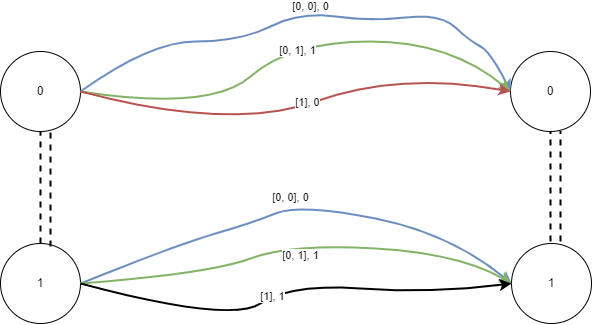
\includegraphics[scale=0.5]{templates/figures/matching-paths-rdni.png}
    \caption{There is no corresponding execution for the red and black executions.}
    \label{fig:RDNI_Matching_Paths}
\end{figure}

We formalized the notion described above to in new definition called \emph{Relatively Deterministic NonInterference} (RDNI). RDNI uses an execution relation that takes a sequence of nondeterministic events, which we call an oracle, and refers to it whenever it needs to make a nondeterministic choice (e.g. crashing or successfully executing). One important requirement is that oracle must capture all the nondeterminism in the system. If all possible nondeterminism in the system is captured by the oracle, it is possible to reason about specific sequence of nondeterministic events by reasoning about the oracle itself. This requirement is enforced by ConFrm while defining execution semantics of a language. Figure \ref{fig:RDNI_no_recovery} shows the formalization of this approach.

%% I took out users from here but will add at the end.
\begin{figure}[ht]
    \centering
    \begin{verbatim}
    Definition simple_RDNI
        {T} (p: prog T)
       (R: state -> state -> Prop) :=
      forall (o: oracle) (s1 s2: state) (res1: Result T),
        exec o s1 p res1 ->
        R s1 s2 ->
        exists res2, 
            exec o s2 p res2 /\
            R (extract_state res1) (extract_state res2) /\
            extract_ret res1 = extract_ret res2.
    \end{verbatim}
    \caption{Simple relatively deterministic noninterference.}
    \label{fig:RDNI_no_recovery}
\end{figure}

Figure \ref{fig:RDNI_no_recovery} states that a program $p$ satisfies \texttt{simple\_RDNI} for any two states $s_1$ and $s_2$ related by $R$, if there is an execution of $p$ from $s_1$ with oracle $o$ that results in $res_1$, then there is an execution of $p$ from $s_2$ with oracle $o$ that with a result $res_2$ such that, states of $res_1$ and $res_2$ are related by $R$, and return values of $res_1$ and $res_2$ are equal.

\subsection{Crash, Reboot, and Recovery}
Since we will be reasoning about crash-safe systems, RDNI should be extended to take crashes, reboots and a recovery into account. We achieve this by changing the execution semantics in the definition with one that captures the entire process of crash-reboot-recovery. There are  important differences in new execution semantics that needs to be explained. 

First is execution relation taking two program arguments, program to run and a recovery program. 

Second is how the state after a crash followed by a reboot handled. Effects of a reboot of a system may be complicated and sometimes even nondeterministic. One example of this is an asynchronous disk. When a system crashes and reboots, the disk can be in one of the multiple possible states nondeterministically due to buffered and reordered writes. To capture and quantify this source of nondeterminism, we introduce  \emph{reboot state functions} \--- or \emph{reboot functions} for short. A reboot function takes a state after a crash and returns the state that the system will be after a reboot. Reboot functions make effects of the reboot on a state deterministic, due to the fact that outcome of a function application is deterministic. Similar to the oracles, different outcomes of a nondeterministic reboot is represented by different reboot functions.

Third is that, execution semantics of a crash-reboot-recovery process must capture multiple crash and recovery attempts. One way to achieve that is providing semantics for execution of the original program followed by the multiple consecutive executions of a recovery program. Since each execution requires an oracle and each crash requires a reboot function to determine after-reboot state, new execution semantics will take a list of oracles and a list of reboot functions. We will explain further details of how executions with recovery implemented in the following section. Figure \ref{fig:RDNI_recovery} shows the formalization with recovery executions.

\begin{figure}[ht]
    \centering
    \begin{verbatim}
Definition RDNI_with_recovery
    {T} (p: prog T) 
    (rec: prog unit)
    (R: state -> state -> Prop) :=
  forall (l_o: list oracle) 
  (l_rf: list (state -> state))
  (s1 s2: state) (res1: Result T),
    exec_with_recovery l_o s1 l_rf p rec res1 ->
    R s1 s2 ->
    exists res2,
        exec_with_recovery l_o s2 l_rf p rec res2 /\
        R (extract_state res1) (extract_state res2) /\
        extract_ret res1 = extract_ret res2.
    \end{verbatim}
    \caption{RDNI with recovery executions.}
    \label{fig:RDNI_recovery}
\end{figure}

{\color{red} One paragraph explaining the changes.}


\subsection{Application specific changes}
There are some application specific changes we made to RDNI. First is the addition of a user to the execution semantics. This change allows us to model multi-user systems and discretionary access control.

Second is conditioning return value equality on a predicate for the user. This way, we can require return value equivalence to hold only for certain users, which is needed to state confidentiality of multi-user systems. For example return value equality is required when the theorem is about adversaries' executions but not needed when it is about normal user's executions.

Third is changing the definition to be about the execution of two programs instead of the same one. This change enables us to reason about functions with different input arguments, because a ConFrm program is a function and its arguments together. 
With these changes, we reach our final definition for RDNI, which is shown in Figure \ref{fig:RDNI_final}.

\begin{figure}[ht]
    \centering
    \begin{verbatim}
    Definition RDNI
        {T} (u: user) (p1 p2: prog T) 
        (rec: prog unit)
       (R: state -> state -> Prop) 
       (cond: user -> Prop):=
      forall (l_o: list oracle) (l_rf: list (state -> state))
      (s1 s2: state) (res1: Result T),
        exec_with_recovery u l_o s1 l_rf p1 rec res1 ->
        R s1 s2 ->
        exists res2,
            exec_with_recovery u l_o s2 l_rf p2 rec res2 /\
            R (extract_state res1) (extract_state res2) /\
            (cond u -> extract_ret res1 = extract_ret res2).
    \end{verbatim}
    \caption{Final definition of RDNI}
    \label{fig:RDNI_final}
\end{figure}


{\color{red}
\subsection{Termination Sensitivity}}

\section{Definitions and Meta-theory}
On top pf RDNI, ConFrm also includes structures and meta-theory that can be used to implement confidential and crash-safe storage systems. This portion consists of two parts, (1) support for abstraction, and (2) the meta-theory that provides relevant theorems to prove confidentiality of implementation from the confidentiality of abstraction. We will first present the infrastructure for defining abstractions and then explain the meta-theory.

\subsection{Abstraction Structures}
\paragraph{Cores.}
ConFrm introduces cores as the main way to model the abstract state of the system and the operations that can be performed on it. A core has four components,
\begin{enumerate}
    \item the state the system
    \item the list of possible operations that can be performed,
    \item the list of possible nondeterminism tokens,
    \item the execution semantics of each operation.
\end{enumerate}

An example core for an in-memory cache can be informally described as
\begin{enumerate}
    \item the state := a partial function from addresses to data
    \item the list of possible operations := \texttt{read}, \texttt{write}, \texttt{evict}, 
    and \texttt{flush}
    \item the list of possible nondeterminism tokens := continue execution, crash here
    \item the execution semantics of each operation := ...
\end{enumerate}.

{\color{red}Explain the example?}

Also, to ensure that tokens capture all the nondeterminism in the semantics, a proof that shows, given a token, execution semantics are deterministic is required.
  
\begin{figure}[ht]
    \centering
    \begin{verbatim}
Record Core :=
  {
    token : Type;
    state : Type;
    operation : Type -> Type;
    exec: forall T, user -> token -> state ->
        operation T -> @Result state T -> Prop;
    
    exec_deterministic_wrt_token :
      forall u o s T (p: operation T) ret1 ret2,
        exec u o s p ret1 ->
        exec u o s p ret2 ->
        ret1 = ret2;
  }.
    \end{verbatim}
    \caption{Definition of a core}
    \label{fig:Core_Definition}
\end{figure}

\paragraph{Crashes.}
ConFrm provides support for crash semantics by defining two different execution results: \texttt{Finished}, and \texttt{Crashed}. A \texttt{Finished} result means that program has successfully completed and contains a state and a return value. A \texttt{Crashed} result means that the program crashed during its execution and contains only a state, which represents the state of the system after the crash happened but before rebooting.

Crash semantics of the system are defined by the developer by defining execution rules that lead to a \texttt{Crashed} result. It is developer's responsibility to ensure that defined execution semantics correctly models the system's both normal and crash behavior.


\paragraph{Languages.}
ConFrm also includes the machinery that turns a core to a full language by equipping it with \texttt{Bind} and \texttt{Return} operations. This eliminates the repetitive work that must to be done to define languages. It also allows framework to provide core-agnostic theorems and tactics to be used in proofs.

Semantics of the language are derived from the semantics of its core. New  semantics takes a list of tokens (i.e., an oracle) and consumes exactly one at each step. 

{\color{red} Some of the Bind/Ret semantics displayed here}

ConFrm also provides some theorems regarding determinism of an execution as well as relationship between oracles and executions like how two executions relate to each other if one's oracle is a prefix of the other's.

\paragraph{Recovery semantics.}
ConFrm provides pre-defined recovery semantics for the systems and adds this semantics automatically when a language is generated from a core. To distinguish recovery semantics from the semantics of the execution of a single program, we will refer to recovery semantics as executing-with-recovery. In ConFrm's recovery model, only two outcomes are possible when executing-with-recovery: (1) execution can finish without any crashes, or (2) execution crashes then recovers after certain number of attempts. To represent these two outcomes, ConFrm uses two types of recovery result: \texttt{RFinished} and \texttt{Recovered}. \texttt{RFinished} corresponds to case (1) and \texttt{Recovered} corresponds to case (2). Since there is no rule for crashing infinitely many times, the provided semantics implicitly assume that recovery eventually will succeed. 

\begin{figure}[ht]
    \centering
    \begin{verbatim}
Inductive exec_with_recovery :
forall T, user -> list oracle -> state -> 
list (state -> state) -> prog T -> prog unit -> 
@Recovery_Result state T -> Prop :=
    | ExecFinished :
      forall T (p: prog' T) p_rec
        u o d d' t,
        exec u o d p (Finished d' t) ->
        exec_with_recovery u [o] d [] p p_rec (RFinished d' t)
    | ExecRecovered :
      forall T (p: prog' T) p_rec
        u o lo d d' get_reboot_state l_grs ret,
        exec u o d p (Crashed d') ->
        exec_with_recovery u lo (get_reboot_state d') 
            l_grs p_rec p_rec ret ->
        exec_with_recovery u (o::lo) d (get_reboot_state::l_grs) 
            p p_rec (Recovered (extract_state ret)).
    \end{verbatim}
    \caption{Recovery semantics in ConFrm}
    \label{fig:Recovery_Semantics}
\end{figure}

Figure \ref{fig:Recovery_Semantics} displays the formal definition.
Semantics for (1) is stated in \texttt{ExecFinished} rule. It is quite straightforward. If the program successfully executes, then it successfully executes-with-recovery.
Semantics for (2) is stated in \texttt{ExecRecovered} rule and more involved. It is inductively defined to capture repeated attempts of recovery until it succeeds. The rule states that, if the original program crashes, and recovery program executes-with-recovery to some result, then original program executes-with-recovery to the state of that result. Execution uses a new oracle and a new reboot function every time a crash-reboot-recovery cycle happens. Therefore, lengths of those lists implicitly determine how many times the recovery will crash until it succeeds.

\paragraph{Refinements.}
ConFrm's main mechanism for relating abstractions and implementations is refinements. 
ConFrm defines a refinement as an object between an implementation language and a core abstracting it. We extend the standard refinement definition to accommodate both crashes and oracles.

As shown in figure \label{fig:Core_Refinement_Definition}, a refinement has four components that corresponds the four components of a core, and a theorem states that a successful execution preserves the state refinement relation. The four components are
\begin{itemize}
    \item a \texttt{compile} function, that turns an  abstract operation to its implementation program,
    \item a \texttt{refines} relation that relates an abstract state to an implementation state,
    \item a \texttt{refines\_reboot} relation that relates an abstract reboot state to an implementation reboot state,
    \item and  \texttt{token\_refines} relation that relates an abstract token to an implementation oracle.
\end{itemize}

\begin{figure}[ht]
    \centering
    \begin{verbatim}
Record CoreRefinement {O_imp} (L_imp: Language O_imp) (O_abs: Core) :=
  {
    compile_core : forall T, O_abs.(Core.operation) T -> L_imp.(prog) T;
    
    refines_core: L_imp.(state) -> O_abs.(Core.state) -> Prop;
    
    refines_reboot_core: L_imp.(state) -> O_abs.(Core.state) -> Prop;
    
    token_refines: forall T, user -> L_imp.(state) -> 
        O_abs.(Core.operation) T -> (L_imp.(state) -> 
        L_imp.(state)) -> L_imp.(oracle) -> 
        O_abs.(Core.token) -> Prop;
    
    exec_compiled_preserves_refinement_finished_core :
      forall T (p2: O_abs.(Core.operation) T) o1 s1 s1' r u,
        (exists s2, refines_core s1 s2) ->
        L_imp.(exec) u o1 s1 (compile_core T p2) (Finished s1' r) ->
        (exists s2', refines_core s1' s2');
  }.
    \end{verbatim}
    \caption{Definition of a core refinement}
    \label{fig:Core_Refinement_Definition}
\end{figure}

Both \texttt{compile} and \texttt{refines} are part of the standard definition. However \texttt{refines\_reboot} and \texttt{token\_refines} relations require more explanation.

We separate \texttt{refines\_reboot} from \texttt{refines} because, in general, \texttt{refines} relation is too strong to hold for after-reboot states but we also needed a relation between them to ensure that recovery restores the original \texttt{refines} relation. {\color{red} Add example here. Cache not having latest value or smth.}

The \texttt{token\_refines} relation is more complicated. On top of the oracle and the token it relates, it takes the following parameters
\begin{itemize}
    \item a user,
    \item an implementation state,
    \item an abstract operation,
    \item and an implementation reboot function.
\end{itemize}
All these parameters are necessary to capture intricate relationship between abstract tokens and implementations' crash and recovery behavior. We can demonstrate the roles they play by examining the following example.

Assume that we are abstracting an implementation of a checksum-based log on an asynchronous disk with a \texttt{write} function.
A crash during a write to a checksum-based log may leave the log in such a state that whether the \texttt{write} succeeded or not would depends on which blocks made it to the disk before crash happened (which is determined by the after-reboot state of the implementation). In other words, success of a write after crash depends on (1) state of the disk just after the crash, and (2) state of the disk after reboot. To determine (1), we need to know the user, the starting state, and data being written, which is in the operation. To determine (2), we need to know the reboot function. Therefore, capturing the behavior of the write in this particular case requires all the parameters listed above. Other operations may require some or all of those parameters as well.

{\color{red} Maybe a figure that demonstrates above paragraph goes here.}

Similar to generating a language from a core, ConFrm can automatically generate a refinement between two languages given a core refinement between an implementation language and an abstraction core. A refinement for a language differs from a refinement for a core in three places. First, \texttt{compile} function transforms programs from the abstraction language to implementation language. Second, \texttt{token\_refines} turns into \texttt{oracle\_refines}, which relates an abstract oracle and an implementation oracle.
Third, a finished execution of any compiled program should preserve the refinement. ConFrm also provides \texttt{recovery\_oracles\_refine} relation, which relates list of implementation oracles to list of abstraction oracles by \texttt{oracle\_refines} inductively.

{\color{red} Refinement picture here.}

\paragraph{Horizontal Compositions.}
To enable modular implementations, ConFrm provides automatic derivation of a new, composite core from two given cores via horizontal composition. State of the composite core is a pair that contains the state of each the component cores. This capability allows developers to develop the system in small, self contained parts that can be combined at will when desired without much overhead. A language derived from a composite ConFrm contains support for "lifting" the programs written in a language of the one of the component cores to the language of the composite core. Similarly, it allows automatic derivation of a refinement between the two composite languages if a component of first language is a refinement of a component of the second language.


\subsection{Meta-theory}
At the heart of ConFrm lies the theorem \ref{fig:RDNI_Transfer_Definition}, which derives the confidentiality of a compiled program from the confidentiality of its abstraction. The theorem reveals sufficient conditions for preserving RDNI through refinement. The two conditions are:

\begin{enumerate}
    \item there should be a simulation between implementation and abstraction with respect to refinement relations, and
    \item if a list of implementation oracles refine a list of abstract oracles from a state with the first program, then it should refine the same oracle from any state that is equivalent to the first state with the second program.
\end{enumerate}

First condition ensures that there is no execution of a compiled program that is not captured by an execution of an abstract program. This is necessary for a property of any abstract execution to imply a property of any implementation execution. If there was an implementation execution that does not correspond to an abstract execution, then it would not be possible to reason about such execution through an abstract execution.

Second condition can be interpreted as the necessity that abstraction does not inject dependency to the confidential data into abstract oracles. Abstractions modelling some deterministic behaviors of an implementation as nondeterminism is a common pattern. For example, an abstraction of a resource allocator may model the allocation function to return an unused resource nondeterministacally, even though the implementation's behavior is actually deterministic. (e.g. returning the first available one). 

This property makes sure that developer does not abstract a behavior that depends on the confidential data in such a way. If such action would be permitted, then two implementation executions from equivalent states with the same implementation oracles could correspond to two abstraction executions with different oracles. In such a case, the noninterference of the abstraction with the same oracles wouldn't be strong enough to establish the same fact in implementation, due to the fact that noninterference of the abstraction does not state anything about executions with different oracles. Formalization of this condition can be seen in figure \ref{fig:ORS_Definition}.

{\color{red} Give example for above paragraph.}

\begin{figure}[ht]
\centering
\begin{verbatim}
Definition oracle_refines_same_from_equivalent
    (u: user) {T} (p1_abs p2_abs: L_abs.(prog) T)
    rec_abs l_get_reboot_state_imp
    (equivalent_states_abs: L_abs.(state) -> L_abs.(state) -> Prop) :=
    
forall l_o_imp l_o_abs l_o_abs' s1_imp s2_imp,

    refines_equivalent equivalent_states_abs s1_imp s2_imp ->

    recovery_oracles_refine 
        u s1_imp p1_abs rec_abs 
        l_get_reboot_state_imp 
        l_o_imp l_o_abs ->

    recovery_oracles_refine 
        u s2_imp p2_abs rec_abs 
        l_get_reboot_state_imp 
        l_o_imp l_o_abs' ->

    recovery_oracles_refine 
        u s2_imp p2_abs rec_abs 
        l_get_reboot_state_imp 
        l_o_imp l_o_abs.
\end{verbatim}
\caption{Formalization of oracle refinement being independent of confidential data}
\label{fig:ORS_Definition}
\end{figure}

\paragraph{Simulations.}
First condition states that a simulation must exist between the abstraction and the implementation. Since we introduced oracles and crash-and-recovery into execution relations, we modify the standard simulation definition to accommodate those changes. 

As shown in figure \ref{fig:Simulation_Definition}, the first change is that, modified simulation definition has three simulation relations, one for the starting states, one for the end states and one for the oracles. We separate the relation that relates the starting and end state to be able to reason about recovery where the relation that holds at the beginning and at the end are different. 

In our case, they were \texttt{refines\_reboot} and \texttt{refines} relations, respectively. However, we also define a two relation variant to use in definition  \label{fig:RDNI_Transfer_Definition}, where start and end relations are both \texttt{refines} relation.

Second change is that a simulation is defined over an entire execution-with-recovery. This allows simulation relation to be broken temporarily after a crash, as long as it is restored by the recovery process. This change is necessary because crashes may expose states that will never appear during a normal execution. This way, refinement relation can only consider the states that appear during normal execution. How to represent crash states is entirely left to the developer. 

Formal definition of a simulation can be found in figure \ref{fig:Simulation_Definition}. In implementation, we separated existence of a list of abstract oracles and existence of an abstract execution separate to shorten the proof scripts for individual theorems.   

\begin{figure}[ht]
\centering
\begin{verbatim}
Definition Simulation
   u T (p_abs: L_abs.(prog) T) (rec_abs : L_abs.(prog) unit)
   l_get_reboot_state_imp
   l_get_reboot_state_abs
   R_begin R_end :=
   
  forall l_o_imp s_imp  s_imp' s_abs,
    R_begin s_imp s_abs ->
   L_imp.(exec_with_recovery) u l_o_imp s_imp
    l_get_reboot_state_imp (R.(compile) p_abs)
    (R.(compile) rec_abs) s_imp' ->
    exists l_o_abs s_abs',
        recovery_oracles_refine u s_imp p_abs rec_abs l_get_reboot_state_imp l_o_imp l_o_abs /\
        L_abs.(exec_with_recovery) u l_o_abs s_abs l_get_reboot_state_abs p_abs rec_abs s_abs' /\
        R_end (extract_state_r s_imp') (extract_state_r s_abs') /\
        extract_ret_r s_imp' = extract_ret_r s_abs').
\end{verbatim}
\caption{ConFrm's simulation relation with oracles and execution-with-recovery}
\label{fig:Simulation_Definition}
\end{figure}


\begin{figure}[ht]
\centering
\begin{verbatim}
Lemma RDNI_transfer:
  forall O_imp O_abs (L_imp: Language O_imp) (L_abs: Language O_abs) 
    (R: Refinement L_imp L_abs)
    u T (p1_abs p2_abs: L_abs.(prog) T) rec_abs
    l_get_reboot_state_imp
    l_get_reboot_state_abs
    equivalent_states_abs cond,

    RDNI
      u p1_abs p2_abs rec_abs
      equivalent_states_abs
      cond l_get_reboot_state_abs ->
    
    Simulation R 
      u p1_abs rec_abs 
      l_get_reboot_state_imp
      l_get_reboot_state_abs ->

    Simulation R 
      u p2_abs rec_abs 
      l_get_reboot_state_imp
      l_get_reboot_state_abs ->
    
    oracle_refines_same_from_equivalent R 
      u p1_abs p2_abs rec_abs 
      l_get_reboot_state_imp 
      equivalent_states_abs ->
    
    RDNI
      u (R.(compile) p1_abs)
      (R.(compile) p2_abs)
      (R.(compile) rec_abs)
      (refines_equivalent R equivalent_states_abs)
      cond l_get_reboot_state_imp.
\end{verbatim}
\caption{RDNI transfer theorem}
\label{fig:RDNI_Transfer_Definition}
\end{figure}

%%%% SOme conclusion here
\iffalse
\section{Property Transfers}

\subsection{RDNI transfer}
- Required properties

-- SimulationForProgram
    
-- abstract oracles exist wrt (AOE)

-- oracle refines same from equivalent (ORS)

-- exec compiled preserves validity (Trivial in our case because all of our top states are valid)

-- Termination Sensitive (TS)

\subsection{ORS}
-- have same structure (program flow equivalence) (HSS)

\begin{minted}{coq}
Lemma token_refines_finished_prefix_eq:
forall ...,

token_refines u s1 op1 grs1 o1 t1 ->
token_refines u s2 op2 grs2 o2 t2 ->

exec u s1 o1 (compile op1) (Finished s1' r1) ->
exec u s2 o2 (compile op2) (Finished s2' r2) ->

have_same_structure op1 op2 -> 

(exists s1a,refines s1 s1a) ->
(exists s2a, refines s2 s2a) ->

one_prefix_of_other o1 o2 ->
o1 = o2 /\ t1 = t2.
\end{minted}

\begin{minted}{coq}
Lemma token_refines_crashed_prefix_eq:
forall ...,

token_refines u s1 op1 grs1 o1 t1 ->
token_refines u s2 op2 grs2 o2 t2 ->

exec u s1 o1 (compile op1) (Crashed s1') ->
exec u s2 o2 (compile op2) (Crashed s2') ->

have_same_structure op1 op2 -> 

(exists s1a,refines s1 s1a) ->
(exists s2a, refines s2 s2a) ->

one_prefix_of_other o1 o2 ->
t1 = t2.
\end{minted}

\begin{minted}{coq}
Lemma oracle_refines_impl_eq:
forall ...,
    oracle_refines u s1 p1 imp_reboot_f o1 oa1 ->
    oracle_refines u s2 p2 imp_reboot_f o2 oa2 ->
    
    refines s1 s1a ->
    refines s2 s2a ->
    
    exec u o1 s1 (compile p1) (Finished s1' r1) ->
    exec u o2 s2 (compile p2) (Finished s2' r2) ->
    
    have_same_structure p1 p2 u s1a s2a ->
    
    token_refines_finished_prefix_eq ->
    
    one_prefix_of_other o1 o2 ->
    not_init p1 ->
    not_init p2 ->
    
    o1 = o2 /\ oa1 = oa2.
\end{minted}

\begin{minted}{coq}
Lemma oracle_refines_independent_from_reboot_function:
forall ...,
    exec u o s (compile p) (Finished s' r) ->
    oracle_refines u s p grs o o_abs ->
    forall grs', 
      oracle_refines u s p grs' o o_abs.
\end{minted}

\begin{minted}{coq}
Lemma oracle_refines_prefix_finished_not_crashed:
forall ...,
    oracle_refines u s1 p1 imp_reboot_f o1 oa1 ->
    oracle_refines u s2 p2 imp_reboot_f o2 oa2 ->
    
    refines s1 s1a ->
    refines s2 s2a ->
    
    exec u o1 s1 (compile p1) (Finished s1' r1) ->
    exec u o2 s2 (compile p2) (Crashed s2') ->
    
    have_same_structure p1 p2 u s1a s2a ->
    
    one_prefix_of_other o1 o2 ->
    not_init p1 ->
    not_init p2 ->
    False.
\end{minted}

These are compositional in the sense that proving corresponding properties for 
each operation implies it is true for all programs created from them. 

\subsection{AOE}
\fi